\section{Experimental Evaluation}
\label{sec:exp_imitation}
In this section, we provide experiments to evaluate DIDA in a wide range of tasks.
We first describe the setting of the experiments in \Cref{subsec:setting_exp_imitation} before presenting and discussing the results in \Cref{subsec:results_imitation}.



\subsection{Setting}
\label{subsec:setting_exp_imitation}

For all the tasks except for Trading, we run and average the results for DIDA and the baselines for 10 seeds.
For Trading, we give the details below.

\subsubsection{Tasks}
\label{subsubsec:tasks_imitation}

\noindent\textbf{Pendulum.}\indent As for the previous chapter, we consider the Pendulum environment for its sensitivity to the delay. 
We consider constant delays in the set $\{3, 5, 10, 15, 20\}$.
For this task, we performed 500 epochs of 5,000 steps each, for a total of 2.5 million steps.

\noindent\textbf{Stochastic Pendulum.}\indent We include the stochastic versions of the Pendulum defined in the previous chapter in order to evaluate DIDA on stochastic environments.
We also consider a constant delay of 5 and we perform 500 epochs of 5,000 steps each, for a total of 2.5 million steps.

\noindent\textbf{Non-integer Delayed Pendulum.}\indent In order to test DIDA on non-integer delays, we propose the following setting. 
First, we learn an undelayed expert with persistence 2, where the persistence represents the number of times the agent repeats an action before being allowed to select a new action \cite{metelli2020control}. 
Basically, with persistence 2, the control frequency of the agent is halved. 
DIDA will then act in states with time steps in the set $(2t)_{t\in\naturalnumbers}$--as does the expert--while the state that DIDA will observe has time steps in $(2t+1)_{t\in\naturalnumbers}$.

\noindent\textbf{Mujoco.}\indent Similarly, we also include the four mujoco environments that are Walker2d, HalfCheetah, Reacher, and Swimmer.
For these tasks, we consider a constant delay of 5 and perform 1,000 epochs of 5,000 steps each, for a total of 5 million steps.

\noindent\textbf{Trading.}\indent In this task, the agent trades the EUR-USD (\texteuro/\$) currency pair on the \gls{fx} at a control frequency of 10 minutes for the period 2016-2019. 
Following the framework of \cite{bisi2020foreign} and \cite{riva2021learning}, it can either \emph{buy}, \emph{sell} or stay \emph{flat} with respect to a fixed amount of USD.
We do not consider trading fees; yet, we take into account the bid-ask spread, which, in practice, has the same effect on the reward as a fee. 
In this framework, we consider a constant action execution delay of 50 seconds.
This results in a non-integer delay.
In this task, we use the years 2016-2017 for the training of the different approaches, 2018 for the validation of the hyperparameters and 2019 for the test. 
A validation set is necessary because the dataset consists of historical data;
the task is a \emph{batch \gls{rl}} or \emph{offline  \gls{rl}} task,  and the approach could overfit the training set. 

\noindent\textbf{Learning Multiple Delays at Once.}\indent For the Pendulum and mujoco environments, we also evaluate the performance of DIDA when trained on higher values of the delay and tested on smaller ones. 
We consider the case of training DIDA for a delay of 10 and testing on smaller delays in $[\![1,9]\!]$ for the Pendulum and similarly for a training delay of 5 for mujoco tasks.


\subsubsection{Baselines}
We consider the baselines used in \Cref{subsubsec:baselines} with the same hyperparameters. 
Namely, these baselines are memoryless \gls{trpo} (M-TRPO), the augmented state \gls{trpo} (A-TRPO), augmented state \gls{sac} (A-SAC),  memoryless \gls{sac} (M-SAC), SARSA and dSARSA with $\lambda=0.9$.
We include the previous approaches L2-TRPO and D-TRPO as well.

We also consider M-DIDA (see~\Cref{subsubsec:dida_no_undelayed_env}) as a baseline to evaluate the necessity to have access to an undelayed environment.

For the Trading task, the undelayed expert used to train DIDA has been selected by validation of its hyperparameters on 2018.
It is also possible to do a validation of its hyperparameters on the delayed dataset for 2018 to select an expert who can better generalise to delays, albeit trained on undelayed data.
We include this baseline in our experiments under the name of ``delayed expert''.

For the Pendulum, we also include BC-DIDA which corresponds to DIDA but where behavioural cloning \cite{bain1995framework} is substituted for \textsc{DAgger} as the imitation algorithm. 
This baseline will be used to study the impact of the choice of an imitation algorithm.


\subsubsection{Setting for DIDA}
\label{subsubsection:our_approach_dida}
In all the experiments, for a fair sample efficiency comparison with other baselines, we include the number of steps that it takes to train the undelayed expert and shift the starting number of samples of DIDA accordingly. 
It is indicated by a vertical dotted line in the figures.
Concerning the undelayed expert itself, we have seen that a smoother expert is beneficial to the performance bound of the imitated delayed policy in \Cref{th:perf_diff_bound}. 
Thus, we consider \gls{sac} as the expert in all the experiments but for the Trading one.  
Indeed, studies on smooth policies \cite{mysore2021regularizing} suggest that the entropy regularised framework of \gls{sac} has a practical effect of learning smoother policies without explicitly optimising for the smoothness of the policy.
For DIDA's policy itself,  we use a simple feed-forward neural network.

For the Trading environment, we leverage the knowledge of an expert trained in years 2016-2017 by Fitted Q-Iteration (FQI)~\cite{ernst2005tree} using XGBoost~\cite{chen2016xgboost} as a regressor for the $Q$ function as in \cite{riva2022addressing}.
In this task, to better match the tree-based approach of the expert, we use Extra Trees~\cite{geurts2006extremely} as a policy for DIDA.
This environment is highly stochastic, and the expert, trained with different seeds, can have very different performances. 
We, therefore, consider 4 experts trained with a different seed but with the same configuration. 
For each expert, we repeat the training of DIDA with 5 seeds.
This sums to a total of 20 trials of DIDA on which the mean and standard deviation of the results are computed. 


For the $\beta$-routine, as suggested by \cite{ross2011reduction}, we set $\beta_1=1, \beta_{i\ge 2}=0$. 
This means that the undelayed expert is used to sample from the environment only at the first iteration of DIDA.


As it can be seen in \Cref{algo:dida}, at each iteration, the buffer of examples for DIDA's training is augmented with the last samples. To prevent the memory from growing infinitely, we use a maximum buffer size of 10 iterations. 
This implies that newer samples overwrite the oldest ones when the buffer is full, in a first-in first-out way.



\subsection{Results}
\label{subsec:results_imitation}

\noindent\textbf{Pendulum.}\indent The returns for the different approaches and for different values of the delay are provided in \Cref{fig:pendulum_varying_delay_imitation}. 
For small delays,  DIDA, BC-DIDA, and M-DIDA achieve comparable returns to A-SAC and slightly better than D-TRPO and L2-TRPO. 
An interesting effect is observed when the delay increases.
Clearly, DIDA and M-DIDA are more robust to an increase in the delay compared with all the other baselines and compared to BC-DIDA whose performance drops sharply.
It is interesting to note the similar performance between DIDA and M-DIDA, which suggests that sampling from an undelayed environment is not a critical element of the algorithm. 
This is confirmed in \Cref{fig:pendulum_imitation} where the result focuses on delay 5, showing the performance as a function of the number of samples. 
DIDA and M-DIDA have very similar learning speeds in terms of sample needed, while BC-DIDA is slightly slower, and so is A-SAC.
The difference in terms of performance between the expert policy and DIDA results from the delay initialization shift problem mentioned in \Cref{subsec:delay_init}. 
In the first steps, in order to initialise the delayed environment in practice, actions are sampled uniformly at random from the environment and can force the agent to start acting while in an unadvantageous state compared to the true initial state.

\begin{figure}[t]
    \centering
    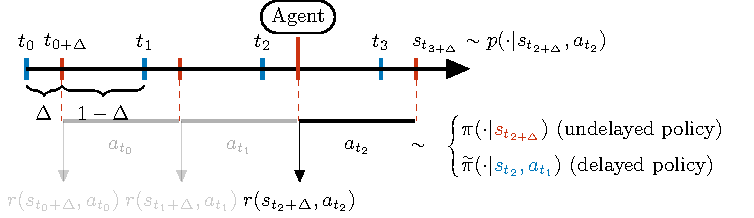
\includegraphics[labelimitation=pendulumvaryingdelay]{img/thesis_plots_imitation.pdf}
    \caption{Mean return of DIDA and baselines for the Pendulum environment for different values of the delay. 
    The horizontal dashed line corresponds to the undelayed expert's (\gls{sac}) performance. 
    Shaded areas represent one standard deviation and the results are obtained for 10 seeds.}
    \label{fig:pendulum_varying_delay_imitation}
\end{figure}

\begin{figure}[t]
    \centering
    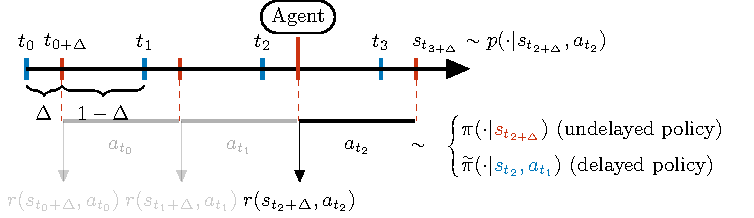
\includegraphics[labelimitation=delay5pendulumimitation]{img/thesis_plots_imitation.pdf}
    \caption{Return obtained by DIDA and benchmarks on the Pendulum environment for a delay of 5. 
    The horizontal dashed line corresponds to the expert's return and the vertical dotted line indicates the number of steps used for training the expert. 
    Shaded areas represent one standard deviation and the results are obtained for 10 seeds.}
    \label{fig:pendulum_imitation}
\end{figure}

\noindent\textbf{Stochastic Pendulum.}\indent We provide the results for these tasks in \Cref{fig:noise_pendulum_imitation}. 
As in the previous chapter, the noises are divided into groups following \Cref{tab:noises}.
For the figure on the top left, all the noises are based on beta distributions. 
On this task, DIDA achieves a much better final performance than the baselines but also converges much faster to these performances.
For the second group in the top right figure, the baselines achieve performance closer to DIDA yet DIDA remains significantly above. 
Finally, for the third group in the bottom left figure, DIDA again achieves the best performance. 
For the LogNormal(1.0) noise the performance significantly drops even for DIDA, this is expected as the noise is strongly asymmetric, which makes the belief distribution more challenging for the algorithms. 

\begin{figure}[t]
    \centering
    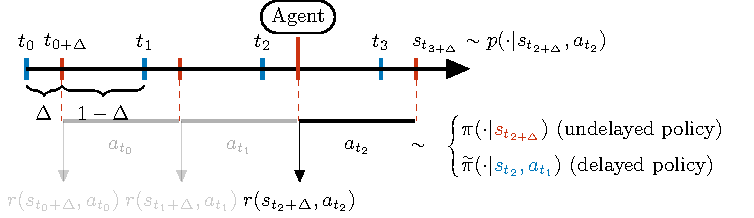
\includegraphics[labelimitation=pendulumnoiseimitation]{img/thesis_plots_imitation.pdf}
    \caption{Return obtained by DIDA and baselines for the Pendulum environment to which are added different noises as explained in \Cref{tab:noises}. 
    The colour indicates noise and the marker indicates the algorithm.
    The horizontal dashed lines indicate the experts' returns for each type of noise and the vertical dotted line indicated the number of steps used for training the expert.
    In the top right figure, the experts' performances are confounded.
    The shaded area indicates one standard deviation and the results are obtained for 10 seeds.}
    \label{fig:noise_pendulum_imitation}
\end{figure}

\noindent\textbf{Non-integer Delayed Pendulum.}\indent The results are provided in \Cref{fig:pendulum_non_int_imitation}.
On this task, DIDA's performance is slightly lower than its performance on integer delays reported in \Cref{fig:pendulum_varying_delay_imitation}. 
There are two explanations for it. 
First, the expert is trained with persistence 2 and has a slightly lower return.
Second, here DIDA is persisting its actions for 2 steps and the delay is therefore doubling in value as well. 
A delay of one in \Cref{fig:pendulum_non_int_imitation} corresponds to a delay of two in \Cref{fig:pendulum_varying_delay_imitation}. 
Anyhow, the performances of DIDA are still satisfactory and show that it can efficiently adapt to non-integer delays.

\begin{figure}[t]
    \centering
    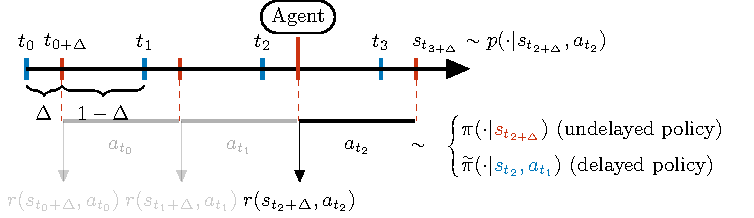
\includegraphics[labelimitation=pendulumnonint]{img/thesis_plots_imitation.pdf}
    \caption{Mean return of DIDA for the Pendulum environment for different values of a non-integer delay. 
    The horizontal dashed line indicates the undelayed expert's (\gls{sac}) performance. 
    Shaded areas represent one standard deviation and the results are obtained for 10 seeds.}
    \label{fig:pendulum_non_int_imitation}
\end{figure}

\noindent\textbf{Mujoco.}\indent The results are presented in \Cref{fig:mujoco_imitation}. 
Here again, DIDA and M-DIDA achieve similar performances while outperforming all the baselines.  
Partly due to the delay's initialization shift, in HalfCheetah and Reacher DIDA performs much worse than the undelayed expert.
More surprisingly, in Swimmer, it performs slightly better.
This is an unexpected implication of the delay's initialization shift.
In fact, in some environments, the initial random sequence of actions could place the agent in a favourable state. 
In HalfCheetah, the random actions sometimes place the agent head-down and the latter thus has to first get back on its feet before moving. In Swimmer, however, the random actions give some initial speed to the agent.

\begin{figure}[t]
    \centering
    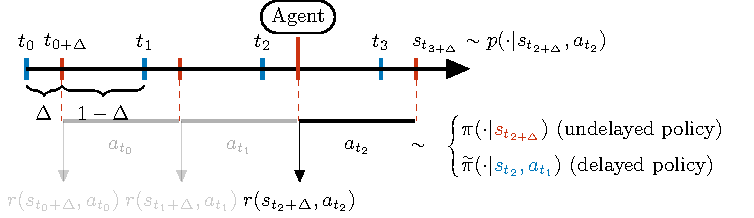
\includegraphics[labelimitation=delay5mujocoimitation]{img/thesis_plots_imitation.pdf}
    \caption{Return obtained by DIDA and benchmarks for various Mujoco environments. 
    The horizontal dashed line corresponds to the expert's return and the vertical dotted line indicates the number of steps used for training the expert. 
    Shaded areas represent one standard deviation and the results are obtained for 10 seeds.}
    \label{fig:mujoco_imitation}
\end{figure}

\noindent\textbf{Trading.}\indent For this task, we report the results obtained in the training set (2019) in \Cref{fig:trading_dida}.
Given the presence of the bid-ask spread, which has a decisive impact on the return, obtaining only a positive return is an achievement. 
DIDA not only achieves a positive return but also clearly outperforms the delayed expert.
A surprising point is that DIDA initially gets a better return than the expert itself. 
The policy is in fact slightly different.
In \Cref{fig:allocation}, we analyse the policy learnt by DIDA by representing the patterns of its actions compared to that of the expert.  
Specifically, this figure illustrates the difficulty of the Batch RL setting. 
The policy learnt by DIDA at the 10$^{\text{th}}$ iteration is very similar to the expert on the training set but starts shifting away from the testing one.

\begin{figure}[t]
    \centering
    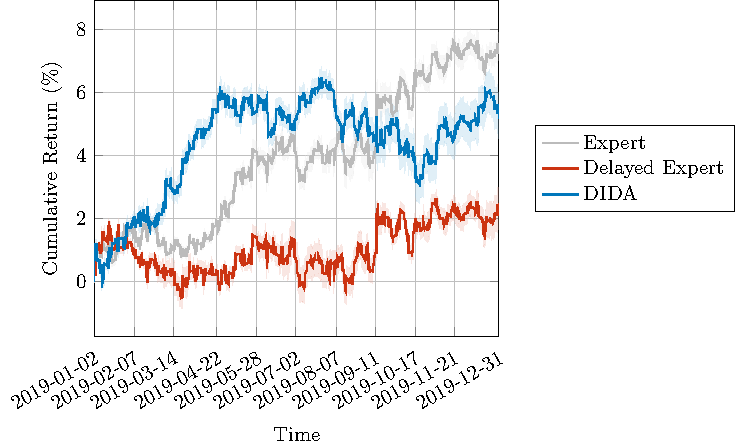
\includegraphics[labelimitationtrading=didatradingeurusd]{img/thesis_plots_chapter_imitation_trading.pdf}
    \caption{Cumulative return, as a percentage of the invested amount, for the trading of the EUR-USD pair in 2019. 
    DIDA is compared against the expert on which it has been trained and to an undelayed expert whose hyperparameters have been selected on a delayed dataset (called ``delayed expert'').}
    \label{fig:trading_dida}
\end{figure}


\begin{figure*}[t]
\centering
    \begin{subfigure}{0.33\textwidth}
        \centering
        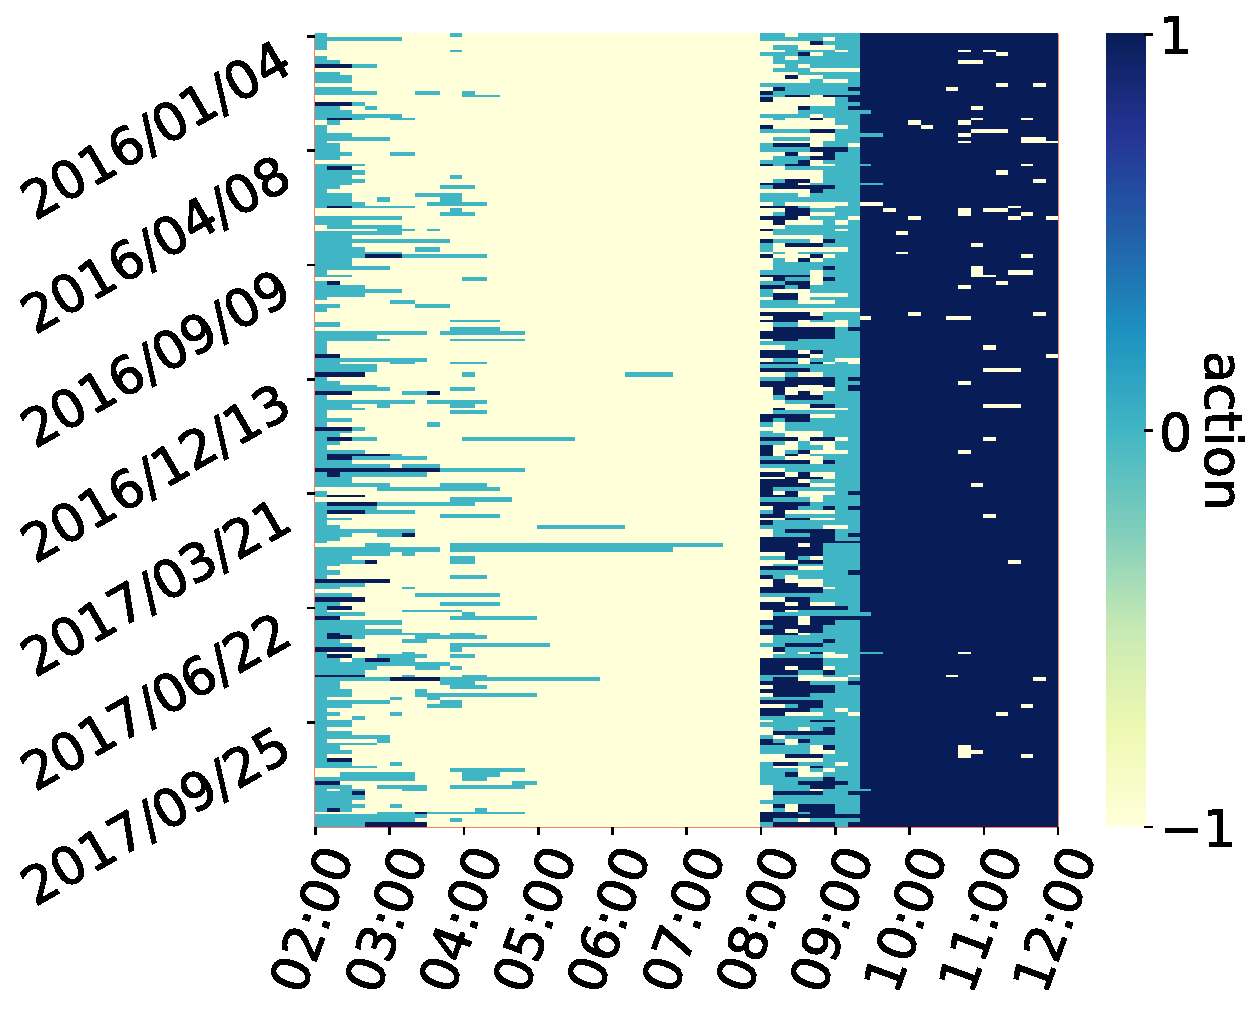
\includegraphics[width=\linewidth]{img/imitation/expert_2016_2017_regular_shift50_expite_10_expseed_0_allocations.pdf}
        \caption{Expert, 2016-2017.}
        \label{fig:test_expert_fx_allocation}
    \end{subfigure}%
\hfill
    \begin{subfigure}{0.33\textwidth}
        \centering
        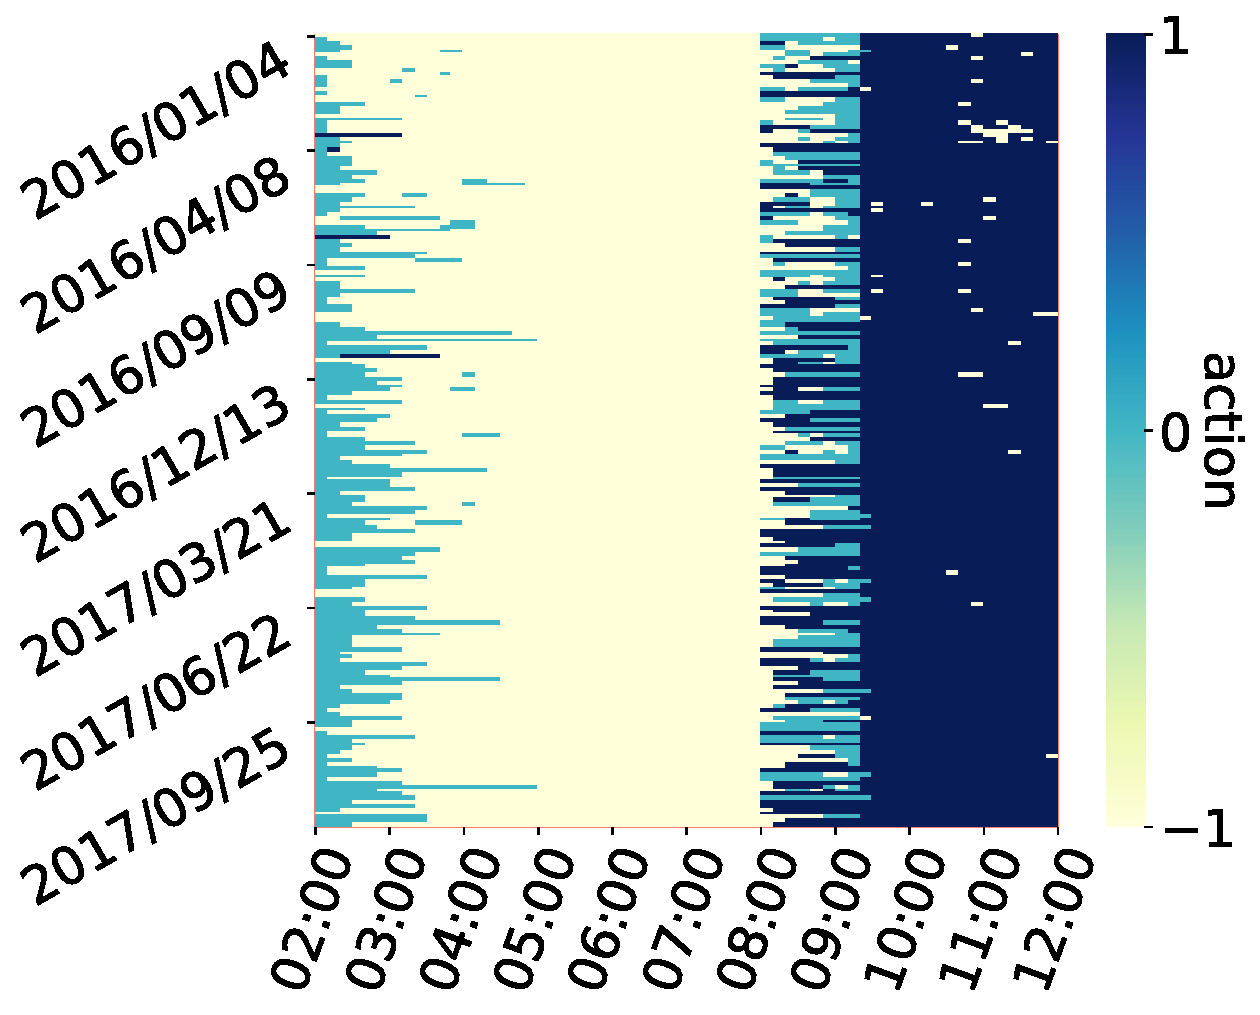
\includegraphics[width=\linewidth]{img/imitation/dida_ms100_est100_shift50_2016_2017_expite_10_expseed_0_dagite_10_dagseed1_allocations.pdf}
        \caption{DIDA, 2016-2017.}
        \label{fig:train_dida_fx_allocation}
    \end{subfigure}%
    \begin{subfigure}{0.33\textwidth}
        \centering
        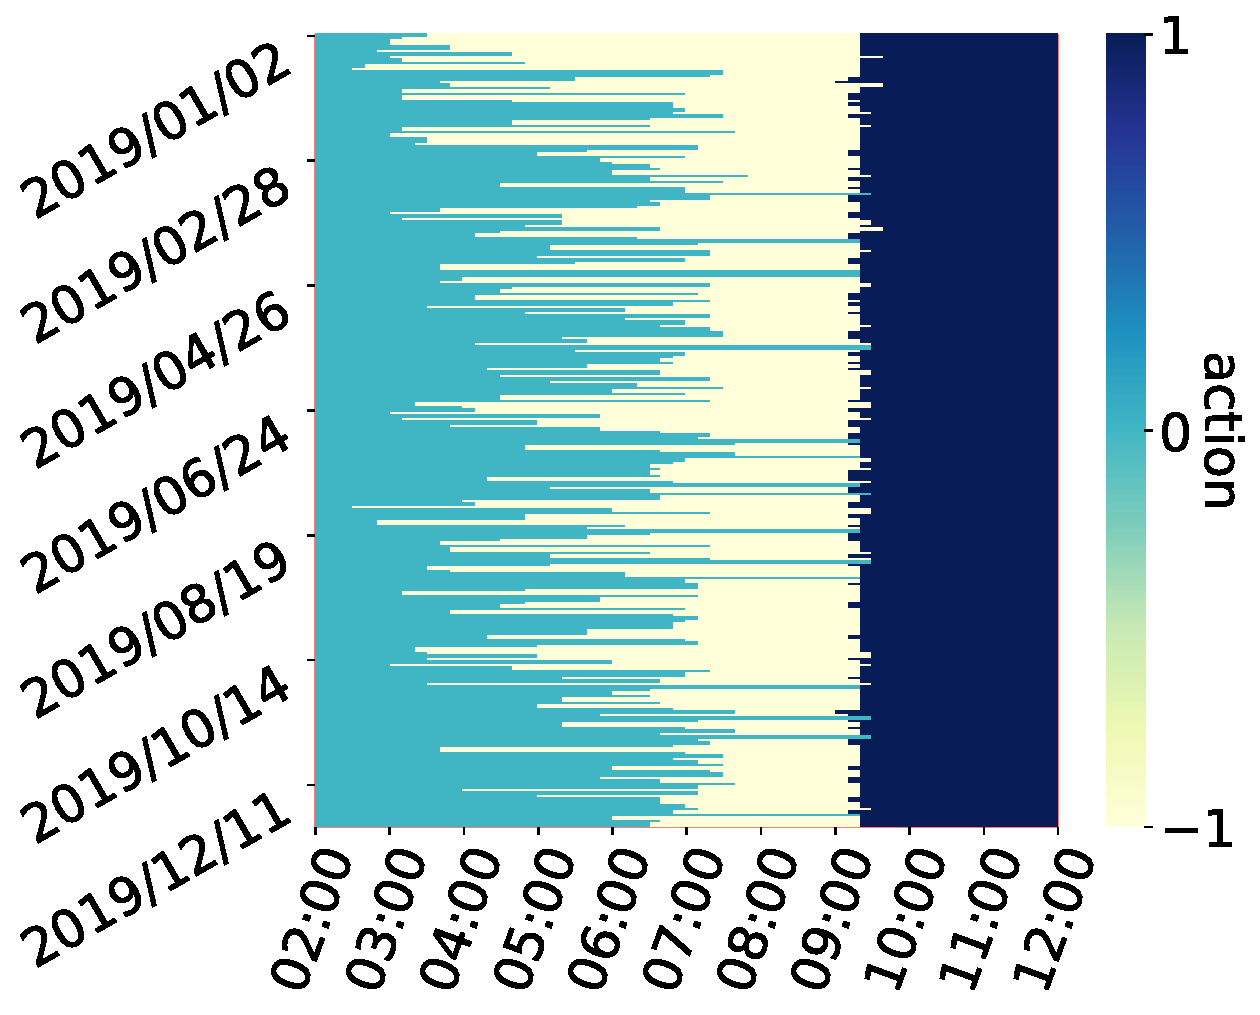
\includegraphics[width=\linewidth]{img/imitation/dida_ms100_est100_shift50_2019_expite_10_expseed_0_dagite_10_dagseed1_allocations.pdf}
        \caption{DIDA, 2019.}
        \label{fig:test_dida_fx_allocation}
    \end{subfigure}%
\caption{Heatmaps representing the patterns in the actions selected by the expert and DIDA on the Trading task.
The expert action patterns (left) are compared to the one of DIDA at the 10th iteration, either on the training set (2016-2017, middle) or on the testing set (2019, right).
The heatmaps show the action (colour) selected for a given minute (column) of a given day (row).}
\label{fig:allocation}
\end{figure*}

\noindent\textbf{Learning Multiple Delays at Once.}\indent Here, we explore the idea presented in \Cref{subsubsec:multi_delay_once_imitation} to apply the policy learnt by DIDA on some delay $\delay>0$ to a smaller delay $0<\delay'<\delay$. 
In \Cref{fig:pendulum_multi_delay_imitation}, we provide the results obtained for the Pendulum task where DIDA's policy is trained on delay $\delay=10$.
In \Cref{fig:mujoco_multi_delay_imitation}, we provide the results obtained for the mujoco tasks where DIDA's policy is trained on delay $\delay=5$.
Clearly and as expected, the performance obtained for smaller delays is similar to the performance reached by DIDA for the delay used during training.



\begin{figure}[t]
    \centering
    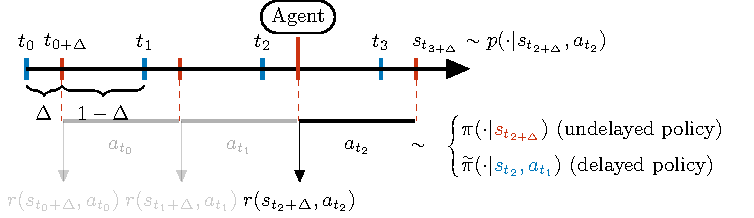
\includegraphics[labelimitation=multipledelayspendulumimitation]{img/thesis_plots_imitation.pdf}
    \caption{Return obtained by a DIDA trained with delay 10 and tested on smaller delays on Pendulum.}
    \label{fig:pendulum_multi_delay_imitation}
\end{figure}

\begin{figure}[t]
    \centering
    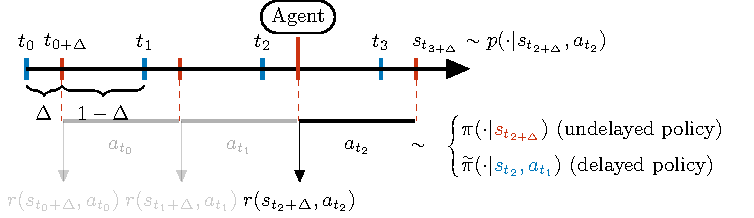
\includegraphics[labelimitation=multipledelaysmujocoimitation]{img/thesis_plots_imitation.pdf}
    \caption{Return obtained by a DIDA trained with delay 5 and tested on smaller delays for various Mujoco environments.}
    \label{fig:mujoco_multi_delay_imitation}
\end{figure}